\chapter{三种期权模型的统一求解框架}\label{chap:method}

本章介绍三种期权模型的统一求解框架的完整设计。核心思路是：通过软掩码机制将BSM、CEV、Heston三种期权模型的PDE算子统一为单一参数化形式，以加法参数化输出解决深度虚值区域的数值退化问题，并引入LLM路由层支持自然语言输入。图~\ref{fig:architecture}给出了系统的三层架构概览。

\begin{figure}[htbp]
  \centering
  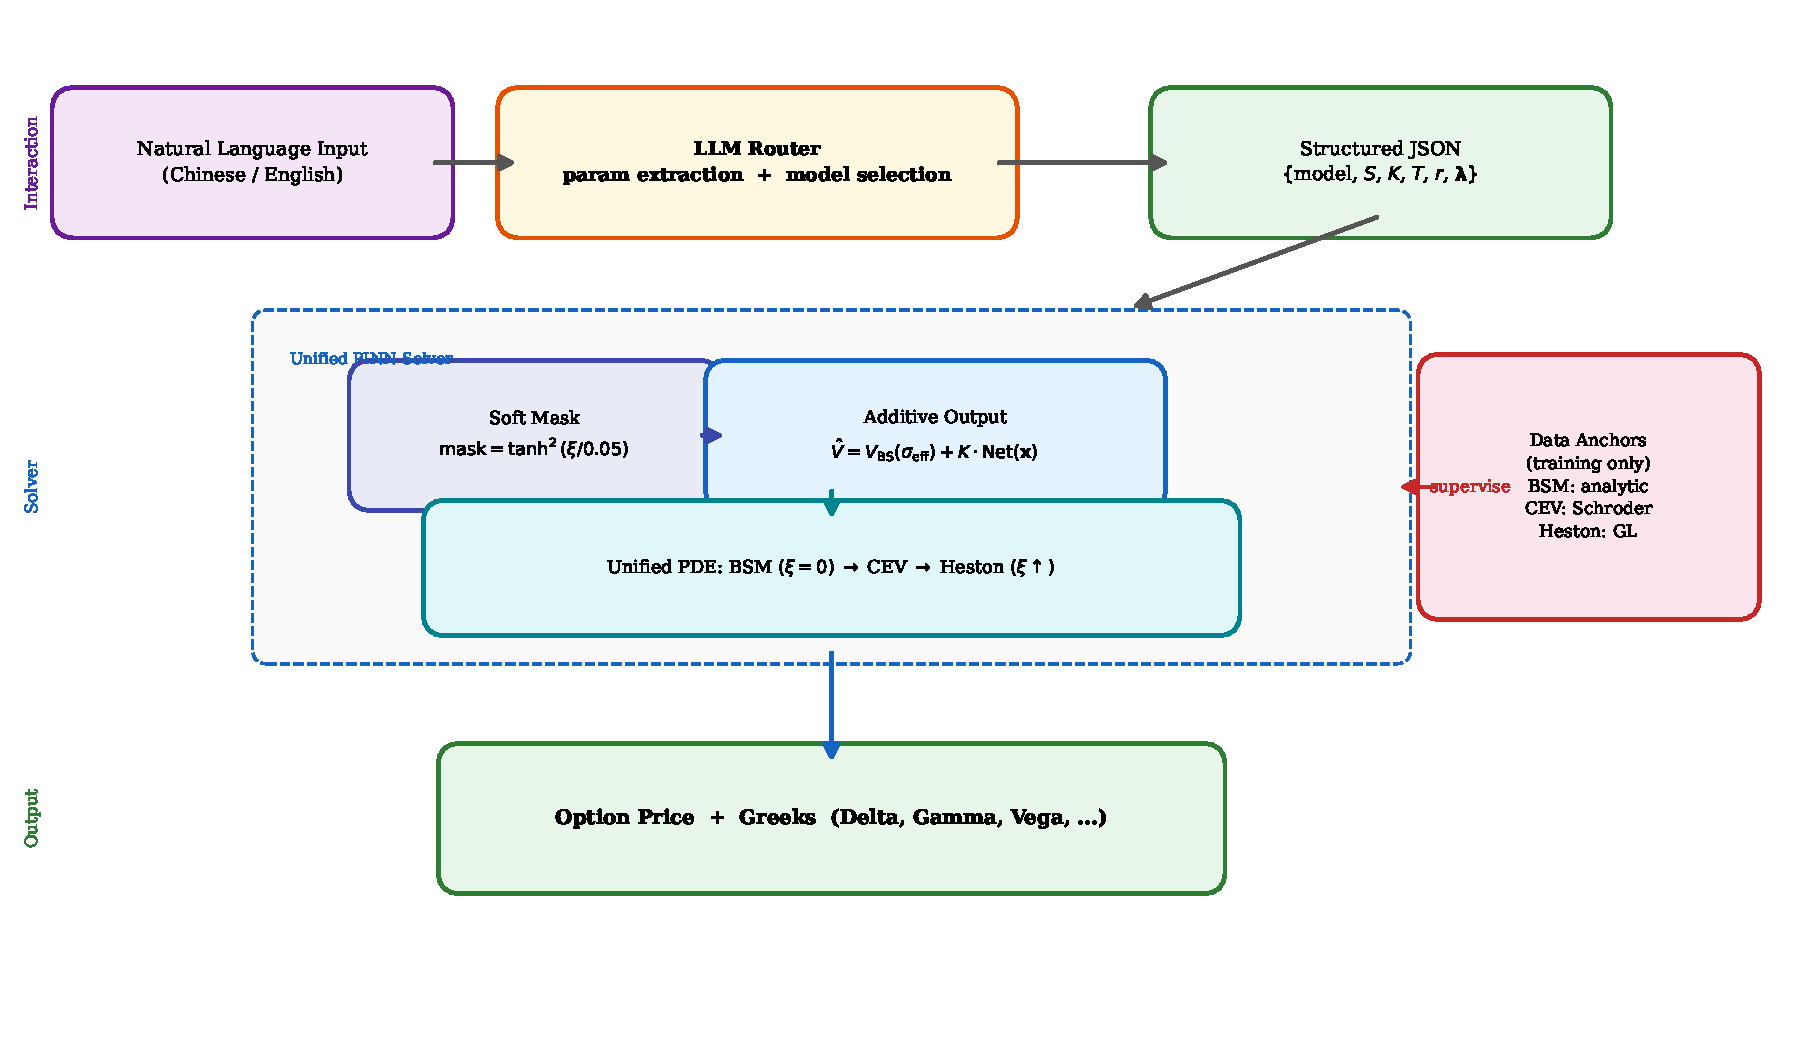
\includegraphics[width=\textwidth]{Img/architecture.pdf}
  \caption{三模型期权定价系统三层架构。交互层：用户以自然语言输入期权需求，LLM路由层提取参数并选择模型，输出结构化JSON。求解层：三模型PINN求解器通过软掩码（$\mathrm{mask}=\tanh^2(\xi/0.05)$）和加法参数化（$\hat{V}=V_\mathrm{BS}(\sigma_\mathrm{eff})+K\cdot\mathrm{Net}(\mathbf{x})$）统一三种期权模型PDE，训练时以解析解/半解析解作为数据锚点。输出层：单次前向传播（$\sim$2\,ms）返回期权价格及Greeks。}
  \label{fig:architecture}
\end{figure}

\section{基于PDE方程的期权定价模型}\label{sec:three_models}

本文涉及的三大期权定价模型均以偏微分方程为核心，其结构差异正是统一框架设计的出发点。BSM模型（式~\eqref{eq:bsm}）以常数波动率$\sigma$为唯一随机性来源，存在封闭解析解，本文将其作为加法参数化的基线：
\begin{align}
  V_\text{BS}(S,\tau;\sigma) &= S\Phi(d_1) - Ke^{-r\tau}\Phi(d_2), \label{eq:bs_formula_ch3}\\
  d_1 &= \frac{\ln(S/K)+(r+\sigma^2/2)\tau}{\sigma\sqrt{\tau}}, \quad d_2 = d_1 - \sigma\sqrt{\tau}.
\end{align}
CEV模型（式~\eqref{eq:cev}）将扩散系数推广为$\sigma^2 S^{2\beta}$，本文取$\beta=0.5$，以Schroder非中心卡方解析解作为数据锚点。Heston模型（式~\eqref{eq:heston}）引入随机方差$v$，PDE升至二维，以特征函数半解析解作为数据锚点。

三种期权模型的PDE均可写为如下统一算子：
\begin{equation}\label{eq:unified_pde}
  \mathcal{F}[V] =
    \frac{\partial V}{\partial t}
    + \frac{1}{2}a(S,v;\boldsymbol{\lambda})\frac{\partial^2 V}{\partial S^2}
    + b(S,v;\boldsymbol{\lambda})\frac{\partial^2 V}{\partial S\partial v}
    + \frac{1}{2}c(v;\boldsymbol{\lambda})\frac{\partial^2 V}{\partial v^2}
    + rS\frac{\partial V}{\partial S}
    + d(v;\boldsymbol{\lambda})\frac{\partial V}{\partial v}
    - rV = 0,
\end{equation}
其中参数向量$\boldsymbol{\lambda}=(\sigma,\beta,\kappa,\theta,\xi,\rho)$控制各系数，具体对应关系如表~\ref{tab:unified_coefficients}所示。

\begin{table}[htbp]
  \centering
  \caption{统一PDE算子系数与三种期权模型的对应关系}
  \label{tab:unified_coefficients}
  \begin{tabular}{lcccc}
    \hline
    模型 & $a(S,v;\boldsymbol{\lambda})$ & $b(S,v;\boldsymbol{\lambda})$ & $c(v;\boldsymbol{\lambda})$ & $d(v;\boldsymbol{\lambda})$ \\
    \hline
    BSM    & $\sigma^2 S^2$    & $0$          & $0$         & $0$ \\
    CEV    & $\sigma^2 S^{2\beta}$ & $0$      & $0$         & $0$ \\
    Heston & $vS^2$            & $\rho\xi vS$ & $\xi^2 v$   & $\kappa(\theta-v)$ \\
    \hline
  \end{tabular}
\end{table}

为实现三种期权模型之间的连续插值，本文引入软掩码：
\begin{equation}\label{eq:soft_mask}
  \text{mask} = \tanh\!\left(\frac{\xi}{0.05}\right)^2.
\end{equation}
利用软掩码，统一PDE算子的各系数具体实现为：
\begin{align}
  a &= (1-m)\cdot\sigma^2 S^{2\beta} + m\cdot vS^2, \label{eq:coeff_a}\\
  b &= m\cdot\rho\xi vS, \label{eq:coeff_b}\\
  c &= m\cdot\xi^2 v, \label{eq:coeff_c}\\
  d &= m\cdot\kappa(\theta-v). \label{eq:coeff_d}
\end{align}
当$\xi=0$时，$m=0$，$b=c=d=0$，$a=\sigma^2 S^{2\beta}$，精确退化为BSM/CEV扩散项；当$\xi\geq 0.3$时，$m\approx 0.998$，$a\approx vS^2$，精确对应Heston扩散项。

\begin{figure}[htbp]
  \centering
  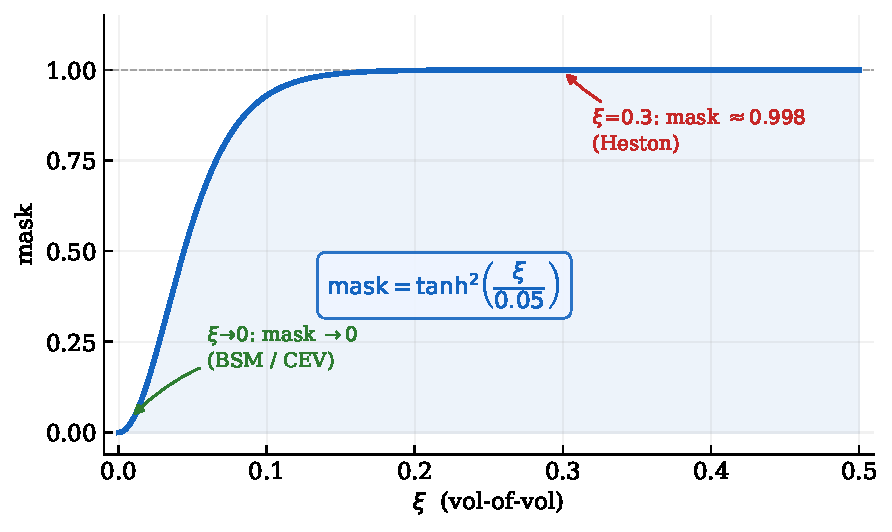
\includegraphics[width=0.75\textwidth]{Img/soft_mask.pdf}
  \caption{软掩码函数$\mathrm{mask}=\tanh^2(\xi/0.05)$随vol-of-vol参数$\xi$的变化。$\xi\to 0$时mask趋近于0，扩散系数退化为BSM/CEV形式；$\xi=0.3$时mask$\approx 0.998$，对应Heston随机波动率结构。函数在$[0,0.5]$区间内单调平滑过渡，避免硬切换引起的梯度不连续。}
  \label{fig:soft_mask}
\end{figure}

软掩码的连续插值特性使网络可以学习到平滑的参数依赖关系，避免了硬切换在$\xi$附近产生的梯度不连续问题（消融实验见第~\ref{sec:ablation}节）。

\section{PINN训练方法}\label{sec:training}

\subsection{网络架构与加法参数化输出}

直接用神经网络输出期权价格存在初始化困难的问题：随机初始化的网络输出量级约为 $10^{-1}$，而期权价格量级约为 $10^0$ 至$10^2$，需要大量训练步数才能收敛到合理区间。一种自然的改进是以 Black-Scholes 解析解为基线，采用乘法参数化 $V = V_{BS}\cdot(1+\text{net})$；然而，深度虚值区域 $V_{BS}\to 0$ 时，乘法修正量随之退化为零，网络对该区域完全失去表达能力。为此，本文采用加法参数化输出：
\begin{equation}\label{eq:additive}
  \hat{V}(S,v,t;\boldsymbol{\lambda}) = V_\text{BS}(S,\tau;\sigma_\text{eff}) + K\cdot\text{net}(x),
\end{equation}
其中等效波动率通过软掩码计算：
\begin{equation}\label{eq:sigma_eff}
  \sigma_\text{eff} = (1-\text{mask})\cdot\sigma + \text{mask}\cdot\sqrt{v}.
\end{equation}
$\sigma_\text{eff}$的设计原则是：对于BSM/CEV输入（$\xi=0$），$\text{mask}=0$，$\sigma_\text{eff}=\sigma$，且$v=v_0=\sigma^2$，Black-Scholes基线即为精确解，网络修正量$K\cdot\text{net}$理想情况下应为零；对于Heston输入（$\xi>0$），$\text{mask}\to 1$，$\sigma_\text{eff}=\sqrt{v}$，Black-Scholes基线提供合理的价格量级初始化，深度虚值时$V_\text{BS}\to 0$，但$K\cdot\text{net}$仍可输出非零修正，网络得以学习Heston相对于BSM基线的价格差异。网络最后一层权重初始化为$\mathcal{N}(0,0.001^2)$，使训练初期$K\cdot\text{net}\approx 0$，两种情形下均从接近正确答案的位置开始优化。

网络输入为9维向量$\mathbf{x}\in\mathbb{R}^9$，各维度的含义与归一化方式如表~\ref{tab:input_encoding}所示。

\begin{table}[htbp]
  \centering
  \caption{三模型PINN网络输入编码}
  \label{tab:input_encoding}
  \begin{tabular}{clccc}
    \hline
    维度 & 变量 & 归一化 & BSM/CEV取值 & Heston取值 \\
    \hline
    1 & $S/S_\text{max}$ & $[0,1]$ & $S/300$ & $S/300$ \\
    2 & $v/v_\text{max}$ & $[0,1]$ & $v_0/1$ & $v/1$ \\
    3 & $t/T$            & $[0,1]$ & $t/T$   & $t/T$ \\
    4 & $\sigma$         & 原始值  & $\sigma$ & $0$ \\
    5 & $\beta$          & 原始值  & $1.0$（BSM）/$0.5$（CEV） & $0$ \\
    6 & $\kappa$         & 原始值  & $0$     & $\kappa$ \\
    7 & $\theta$         & 原始值  & $0$     & $\theta$ \\
    8 & $\xi$            & 原始值  & $0$     & $\xi$ \\
    9 & $\rho$           & 原始值  & $0$     & $\rho$ \\
    \hline
  \end{tabular}
\end{table}

归一化策略的设计原则是：状态变量$S$和$v$的量级差异较大（$S\in[0,300]$，$v\in[0,1]$），归一化至$[0,1]$可避免梯度方向因量级悬殊而失衡；时间维度$t/T$同理归一化至$[0,1]$。模型参数（$\sigma,\beta,\kappa,\theta,\xi,\rho$）直接以原始值输入，保留参数的绝对量级信息，使网络能够感知参数变化对期权价格的影响幅度。BSM/CEV输入时，$\xi=0$与软掩码机制衔接，无需额外的模型标识符即可区分三种模型。
网络采用6层全连接结构，每层128个神经元，激活函数为$\tanh$：
\begin{align}
  h_0 &= x \in \mathbb{R}^9, \\
  h_l &= \tanh(W_l h_{l-1} + b_l), \quad l=1,\ldots,6, \\
  \text{net}(x) &= W_7 h_6 + b_7 \in \mathbb{R}.
\end{align}
$\tanh$激活函数光滑且高阶导数有界，适合PINN中计算二阶偏导数的场景。最后一层权重初始化为$\mathcal{N}(0,0.001^2)$、偏置初始化为0，使训练初期$K\cdot\text{net}\approx 0$，网络输出近似退化为Black-Scholes基线$V_\text{BS}$；在终值处（$t=T$，$\tau=0$）$V_\text{BS}$自动满足$V_\text{BS}(S,0;\sigma_\text{eff})=\max(S-K,0)$，终值条件在训练初期无需额外惩罚即可自然成立，这一设计参考了Guo等人\cite{guo2024icpinn}的ICPINN方法。

\subsection{损失函数与配点采样}

三模型PINN的总损失由PDE残差、边界条件和数据锚点三部分组成：
\begin{equation}\label{eq:total_loss}
  \mathcal{L}(\theta) = w_\text{pde}\,\mathcal{L}_\text{pde}
                      + w_\text{bc}\,\mathcal{L}_\text{bc}
                      + w_\text{data}\,\mathcal{L}_\text{data}.
\end{equation}

配点是PINN训练的核心数据来源，完全由求解域的几何结构决定，无需任何真实市场观测数据。对每个参数变体在求解域$\Omega=[0,S_\text{max}]\times[0,v_\text{max}]\times[0,T]$内均匀随机采样$N_c=5000$个配点，每个训练步骤重新采样（online sampling），避免过拟合到固定配点集。对于BSM/CEV模型，$v$维度退化为常数，配点实际为二维；对于Heston模型，配点为完整三维。边界配点在各边界面上均匀采样$N_b=500$个点。数据锚点在$t=0$处取$N_d=20$个均匀分布的$S$值，对应价格由参考解析解预先计算，这是训练中唯一涉及"真实"（解析）价格的部分。

PDE残差损失在求解域$\Omega=[0,S_\text{max}]\times[0,v_\text{max}]\times[0,T]$内随机采样$N_c$个配点，计算统一PDE算子的相对残差：
\begin{equation}
  \mathcal{L}_\text{pde} = \frac{1}{N_c}\sum_{i=1}^{N_c}
    \left(\frac{\mathcal{F}[\hat{V}](S_i,v_i,t_i)}{|\hat{V}(S_i,v_i,t_i)|+1}\right)^2.
\end{equation}
分母中的$|\hat{V}|+1$为相对归一项，避免ATM区域的残差主导损失，使OTM区域也能获得足够的梯度信号。配点在每个训练步重新采样（online sampling），避免过拟合到固定配点集。

边界条件损失在各边界面上采样$N_b=500$个点，目标值由期权定价的渐近行为决定：下边界$V(0,v,t)=0$（标的价值为零时看涨期权无价值），上边界$V(S_\text{max},v,t)=S_\text{max}-Ke^{-r(T-t)}$（深度实值时期权近似等于持有标的），$v$方向上边界$V(S,v_\text{max},t)\approx S$。边界条件损失为对应目标值的均方误差。

数据锚点损失解决纯PDE约束解不唯一的问题：仅凭PDE和边界条件，方程存在多个满足条件的解，数据锚点损失在$t=0$处以参考解析解为目标：
\begin{equation}
  \mathcal{L}_\text{data} = \frac{1}{N_d}\sum_{j=1}^{N_d}
    \left(\hat{V}(S_j,v_j,0) - V_j^*\right)^2,
\end{equation}
其中$V_j^*$为参考解。$N_d=20$个均匀分布的$S$值。这是训练中唯一涉及解析价格的部分。

损失权重设置为$(w_\text{pde}, w_\text{bc}, w_\text{data})=(1, 10, 100)$，其中$w_\text{data}=100$确保网络在已知解处精确拟合，防止PDE约束将解推向错误方向；消融实验验证了此权重组合的必要性（见第~\ref{sec:ablation}节）。

训练时对72个参数变体（6 BSM + 12 CEV + 54 Heston）同时采样配点：每个训练步骤中，每个参数变体各采样5000个配点，拼接后计算统一PDE残差。这一策略确保网络在三种模型的参数空间中均匀训练，避免某一模型主导损失。对于BSM/CEV模型，$v$维度退化为常数，配点实际为二维；对于Heston模型，配点为完整三维。使用Adam优化器\cite{kingma2014adam}，初始学习率$10^{-3}$，余弦退火学习率调度（$\eta_\text{min}=10^{-5}$），总训练轮数30000轮，在NVIDIA GPU上约需1小时。

\section{LLM路由层}\label{sec:llm_router}

三种定价模型分别适用于不同的市场假设，传统工具要求用户手动指定模型类型和全部数值参数。本文引入DeepSeek LLM作为智能路由层，使用户可以通过自然语言描述期权需求，由LLM自动完成模型选择和参数提取。

系统提示词将LLM角色定义为"期权定价参数提取器"，规定模型选择规则：仅提供$\sigma$则选BSM，提及$\beta$或CEV则选CEV，提供$\kappa,\theta,\xi,\rho,v_0$或提及Heston、stochastic volatility则选Heston，默认BSM。对用户未提及的参数使用典型默认值（$S=100$，$K=100$，$T=1.0$，$r=0.05$，$\sigma=0.2$，$\beta=0.5$，$v_0=0.04$，$\kappa=2.0$，$\theta=0.04$，$\xi=0.3$，$\rho=-0.7$），并通过\texttt{response\_format: json\_object}强制输出合法JSON。LLM的输出遵循以下JSON Schema：
\begin{verbatim}
{
  "model": "bsm" | "cev" | "heston",
  "option_type": "call" | "put",
  "S": float, "K": float, "T": float, "r": float,
  "sigma": float, "beta": float,
  "v0": float, "kappa": float, "theta": float,
  "xi": float, "rho": float
}
\end{verbatim}

系统在接收到JSON输出后，进行参数范围校验（如$\sigma\geq 0$，$\beta\in(0,1]$，$\xi\geq 0$，$\rho\in(-1,1)$），对越界参数截断至合法范围，再传入三模型PINN求解器。对于欧式看跌期权，通过看跌-看涨平价关系转换：
\begin{equation}
  P = C - S + Ke^{-r(T-t)}.
\end{equation}
鲁棒性方面，对于单位歧义（如``到期时间30天"与``到期时间0.082年"），系统提示词要求LLM将所有时间参数统一转换为年为单位输出。对于缺失字段，LLM使用预设默认值填充，不产生空值。本文的LLM路由层定位为教育和研究工具的前端接口，生产环境部署需额外增加规则校验层和审计日志。

完整定价流程为：用户输入自然语言描述（中英文均可）；LLM提取参数并选择模型；三模型PINN加载预训练权重，构造参数向量$\boldsymbol{\lambda}$；网络前向传播返回期权价格（约2ms）。

\section{参数化PINN对比方法}\label{sec:parametric_pinn}

为与三模型PINN在设计路线上形成对比，本文同时实现了一个全参数化PINN（Fully Parametric PINN）作为基准。该方法将所有模型参数$(\sigma,\beta,\kappa,\theta,\xi,\rho)$与合约特征$(S,v,\tau,K,r)$共11维向量直接作为网络输入，采用8层$\times$256神经元的全连接网络，同样使用加法参数化输出$\hat{V}=V_{\mathrm{BS}}(\sigma_{\mathrm{eff}})+K\cdot\mathrm{net}(x)$和软掩码机制。与三模型PINN的主要区别在于：参数化PINN在更宽的参数范围内（BSM：$\sigma\in[0.05,0.50]$；CEV：$\sigma\in[0.10,0.30]$，$\beta\in[0.10,0.90]$；Heston：$\kappa\in[0.5,10]$，$\xi\in[0.05,0.50]$，$\rho\in[-0.95,-0.10]$）随机采样训练，理论上具有更强的参数泛化能力，但网络容量需求更高（参数量约为三模型PINN的4倍）。三模型PINN则针对有限参数变体精确求解，以较小的网络覆盖实用参数范围。

\section{本章小结}\label{sec:method_summary}

本章介绍了三种期权模型的统一求解框架。核心创新在于：（1）软掩码机制将三种期权模型的PDE算子统一为单一参数化形式，实现模型间的连续插值；（2）加法参数化输出以Black-Scholes解析解为基线，解决了深度虚值区域的数值退化问题；（3）LLM路由层通过结构化输出实现可靠的参数提取和模型选择，并支持欧式看涨和看跌期权。下一章将报告实验结果。
